\chapter{Конструкторская часть}

\section{Проектирование базы данных}
В соответствии с выделенными сущностями и связями между ними, показанными на диаграмме сущность-связь, представленной на рисунке~\ref{er_img}, проектируемая база данных должна содержать следующие таблицы:
\begin{itemize}
	\item таблица \textbf{users}, хранящая информацию о пользователях приложения;
	\item таблица \textbf{roles} типов пользователей приложения;
	\item таблица \textbf{drinks} всех напитков, имеющихся в системе;
	\item таблица \textbf{categories}, хранящая категории напитков;
	\item таблица \textbf{drinkscategory}, являющая связующей таблицей между напитком и категорией (формализует связь <<многие--ко--многим>>);
	\item таблица \textbf{favdrinks} избранных напитков (формализует связь <<многие--ко--многим>> между пользователем и напитком);
	\item таблица \textbf{companies}, хранящая информацию о сетях кофеен;
	\item таблица \textbf{menu}, хранящая информацию о меню напитков;
	\item таблица \textbf{loyaltyprograms}, хранящая информацию о программе лояльности сети кофеен;

	\item таблица \textbf{coffeeshops}, хранящая информацию о кофейнях сети;
	\item таблица \textbf{favcoffeeshops} избранных кофеен (формализует связь <<многие--ко--многим>> между пользователем и кофейней).
\end{itemize}

На рисунке~\ref{db_diagram} представлена диаграмма проектируемой базы данных.

\newpage

\begin{figure}[H]
	\centering
	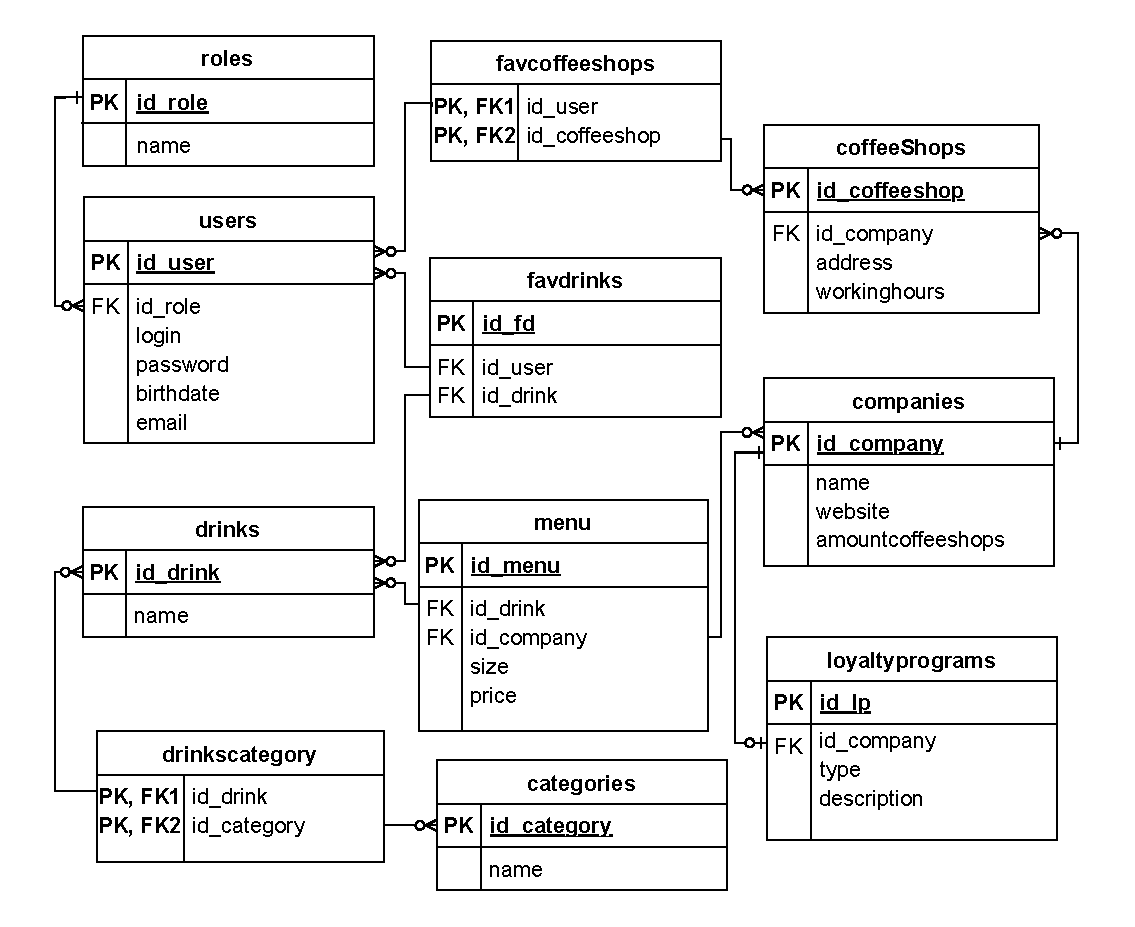
\includegraphics[width=1\linewidth]{img/db_diagram2605.pdf}
	\caption{Диаграмма базы данных}
	\label{db_diagram}
\end{figure}

Таблица \textbf{users} содержит следующие поля:
\begin{itemize}
	\item id\_user -- идентификатор пользователя, первичный ключ;%, UUID;
	\item login -- логин пользователя;% VARCHAR(128);
	\item password -- пароль пользователя; %VARCHAR(128);
	\item birthdate -- дата рождения пользователя;%, DATE;
	\item email -- электронная почта пользователя;%, VARCHAR(256);
	\item id\_role -- идентификатор роли пользователя, внешний ключ.%, INT.
\end{itemize}

Таблица \textbf{roles} содержит следующие поля:
\begin{itemize}
	\item id\_role -- идентификатор роли пользователя, первичный ключ;%, INT;
	\item name -- название роли.%, VARCHAR(128).
\end{itemize}

Таблица \textbf{drinks} содержит следующие поля:
\begin{itemize}
\item id\_drink -- идентификатор напитка, первичный ключ;%, UUID;
\item name -- название напитка.%, VARCHAR(128).
\end{itemize}

Таблица \textbf{categories} содержит следующие поля:
\begin{itemize}
	\item id\_category -- идентификатор категории напитка, первичный ключ;%, UUID;
	\item name -- название категории напитка.%, VARCHAR(128).
\end{itemize}

Таблица \textbf{drinkscategory} содержит следующие поля:
\begin{itemize}
%\item Id\_dc -- первичный ключ, INT;
\item id\_category -- идентификатор категории напитка, внешний ключ;%, UUID;
\item id\_drink -- идентификатор напитка, внешний ключ.%, UUID.
\end{itemize}

Таблица \textbf{favdrinks} содержит следующие поля:
\begin{itemize}
%	\item Id\_fd -- первичный ключ, INT;
	\item id\_user -- идентификатор пользователя, внешний ключ;%, UUID;
	\item id\_drink -- идентификатор напитка, внешний ключ.%, UUID.
\end{itemize}

Таблица \textbf{companies} содержит следующие поля:
\begin{itemize}
	\item id\_company -- идентификатор сети кофеен, первичный ключ;%, UUID;
	\item name -- название сети;%, VARCHAR(128);
	\item website -- веб-сайт;%, VARCHAR(256);
	\item amountcoffeeshops -- количество открытых кофеен сети.%, INT;
\end{itemize}
	
Таблица \textbf{menu} содержит следующие поля:
	\begin{itemize}
		\item id\_menu -- первичный ключ;%, UUID;
		\item id\_drink -- идентификатор напитка, внешний ключ;%, UUID;
		\item id\_company -- идентификатор сети кофеен, внешний ключ;%, UUID;
		\item size -- объем напитка (в миллилитрах);%, INT;
		\item price -- цена (в рублях).%, NUMERIC(10, 2).
\end{itemize}

Таблица \textbf{loyaltyprograms} содержит следующие поля:
\begin{itemize}
	\item id\_lp -- идентификатор программы лояльности, первичный ключ;%, UUID;
	\item id\_company -- идентификатор сети кофеен, внешний ключ;%, UUID;
	\item type -- тип программы лояльности(например, пластиковая карта, мобильное приложение и тд.);%, TEXT.
	\item description -- краткое описание предоставляемых программой лояльности предложений для покупателей.%, TEXT.
\end{itemize}

Таблица \textbf{coffeeshops} содержит следующие поля:
\begin{itemize}
	\item id\_coffeeshop -- идентификатор кофейни, первичный ключ;%, UUID;
	\item id\_company -- идентификатор сети кофеен, внешний ключ;%, UIID;
	\item address -- адрес кофейни;%, VARCHAR(256);
	\item workinghours -- часы работы.%, VARCHAR(64).
\end{itemize}

Таблица \textbf{favcoffeeshops} содержит следующие поля:
\begin{itemize}
%	\item Id\_fcs -- первичный ключ, UUID;
	\item id\_user -- идентификатор пользователя, внешний ключ;%, UUID;
	\item id\_coffeeshop -- идентификатор кофейни, внешний ключ.%, UUID.
\end{itemize}

\section{Ограничения целостности данных}
\subsection{Целостность таблиц}
Для обеспечения целостности таблиц каждая строка должна иметь уникальный идентификатор (первичный ключ). Как было описано в разделе 2.1, каждая из таблиц имеет первичный ключ:
\begin{itemize}
	\item поле id\_role в таблице roles;
	\item поле id\_user в таблице users;
	\item поле id\_drink в таблице drinks;
	\item поле id\_category в таблице categories;
	\item поле id\_company в таблице companies;
	\item поле id\_coffeeshop в таблице coffeeshops;
	\item поле id\_lp в таблице loyaltyprograms;
	\item поле id\_menu в таблице menu;
	\item поля id\_drink и id\_category в таблице drinkscategory (составной первичный ключ);
	\item поля id\_user и id\_drink в таблице favdrinks (составной первичный ключ);
	\item поля id\_user и id\_coffeeshop в таблице favcoffeeshops(составной первичный ключ).
\end{itemize}

\subsection{Целостность полей}
Чтобы обеспечить целостность полей таблицы, следует указать набор допустимых значений для них.

Для таблицы \textbf{roles} необходимо выполнить следующие условия:
\begin{itemize}
 \item поле name может принимать значения <<user>>, <<moderator>>, <<guest>>, <<administrator>>; 
 \item любые поля не должны быть пустыми.%иметь  нулевое значение (<<null>>).
 \end{itemize} 
 
 Для таблицы \textbf{users} необходимо выполнить следующие условия:
 \begin{itemize}
 	\item значение поля login должно быть уникальным, поскольку оно используется для авторизации пользователей;
 	\item значение поля birthdate, хранящее дату рождения пользователя, не должно превышать значение текущей даты;
 	\item любые поля не должны быть пустыми. %иметь нулевое значение(<<null>>).
 \end{itemize}
 
Для таблицы \textbf{drinks} необходимо выполнить следующие условия:
 \begin{itemize}
 	\item поле name должно быть уникальным;
 	\item все поля не могут быть пустыми. %иметь нулевое значение(<<null>>).
 \end{itemize}
 
 Для таблицы \textbf{categories} необходимо выполнить следующие условия:
 \begin{itemize}
 	\item поле name должно быть уникальным;
 	\item все поля не могут быть пустыми. %иметь нулевое значение(<<null>>).
 \end{itemize}
 
Для таблицы \textbf{companies} необходимо выполнить следующие условия:
 \begin{itemize}
 	\item значение поля amountcoffeeshops не может быть отрицательным;
 	\item все поля, кроме поля website, не могут быть пустыми.%иметь нулевое значение(<<null>>).
 \end{itemize}
 
Для таблицы \textbf{menu} необходимо выполнить следующие условия:
\begin{itemize}
	\item значение поля size должно быть > 0;
	\item значение поля price должно быть неотрицательным;
	\item все поля не могут быть пустыми.

\end{itemize}

Для таблицы \textbf{loyaltyprograms} необходимо выполнить следующие условия:
\begin{itemize}
	\item все поля не могут быть пустыми. %иметь нулевое значение(<<null>>).
\end{itemize}

Для всех остальных таблиц необходимо выполнить следующие условия:
\begin{itemize} 
	\item любые поля не должны быть пустыми.%иметь нулевое значение(<<null>>).
\end{itemize}

\subsection{Целостность ссылок}
Связь между таблицами организована с помощью внешних ключей.
%, ссылающихся на соответствующие первичные ключи. 
Для обеспечения ссылочной целостности необходимо, чтобы для каждого значения внешнего ключа, появляющегося в дочерней таблице, в родительской таблице существовал кортеж с таким же значением первичного ключа. В таблице~\ref{fk_table} представлены все внешние ключи таблиц, имеющихся в базе данных.

\newpage
\begin{table}[ht]
	\begin{center}
		\begin{threeparttable}
			\caption{\label{fk_table} Внешние ключи таблиц}
			\begin{tabular}{|p{5cm}|p{4cm}|p{6cm}|c|}
				\hline	
				\textbf{Таблица} & \textbf{Внешний ключ} & \textbf{Таблица, на поле которой ссылается внешний ключ}  \\ \hline
				
				users & id\_role & roles(id\_role) \\ \hline
				
				favdrinks & id\_user & users(id\_user) \\ 
				 & id\_drink & drinks(id\_drink) \\ \hline
				 
				 favcoffeeshops & id\_user & users(id\_user) \\ 
				 & id\_coffeeshop & cofeeshops(id\_coffeeshop) \\ \hline
				 
				 menu & id\_company & companies(id\_company) \\ 
				 & id\_drink & drinks(id\_drink) \\ \hline
				 
				 drinkscategory & id\_category & categories(id\_category) \\ 
				 & id\_drink & drinks(id\_drink) \\ \hline
				 
				 loyaltyprograms & id\_company & companies(id\_company) \\ \hline
			
				
			\end{tabular}
		\end{threeparttable}
	\end{center}
\end{table}

\section{Триггеры}
Для поддержания ссылочной целостности необходимо реализовать следующие триггеры.

Триггер, алгоритм работы которого представлен на рисунке~\ref{trigger_del_drink}, удаляет из таблиц menu, favdrinks и drinkscategory все записи, связанные с удаляемым из таблицы drinks напитком.

\begin{figure}[H]
	\centering
	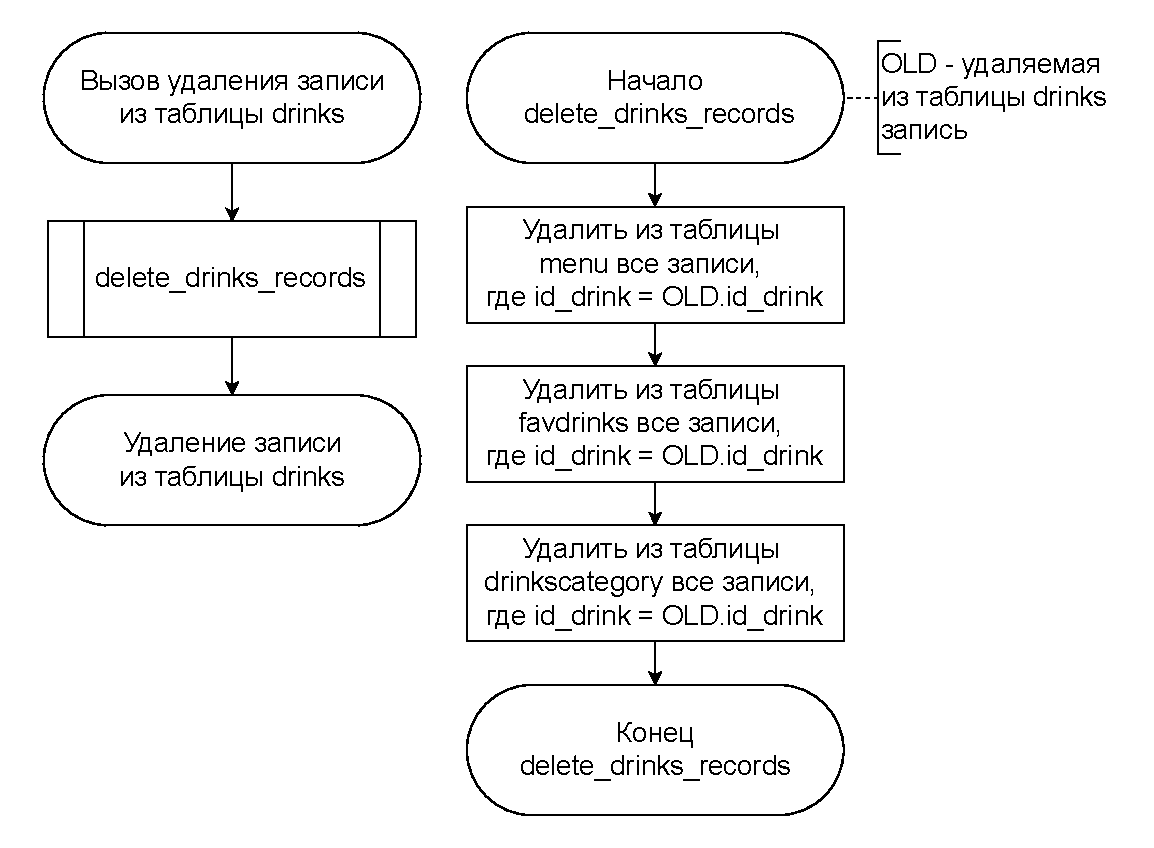
\includegraphics[width=0.7\linewidth]{img/trigger_del_drink.pdf}
	\caption{Триггер на удаление всех записей из таблиц  menu, favdrinks и drinkscategory, связанных с удаляемым из таблицы drinks напитком}
	\label{trigger_del_drink}
\end{figure}


Триггер, удаляющий из таблиц favcoffeeshops и favdrinks все записи, связанные с удаляемым из таблицы users пользователем. Алгоритм работы этого триггера представлен на рисунке~\ref{trigger_del_user}.

\begin{figure}[H]
	\centering
	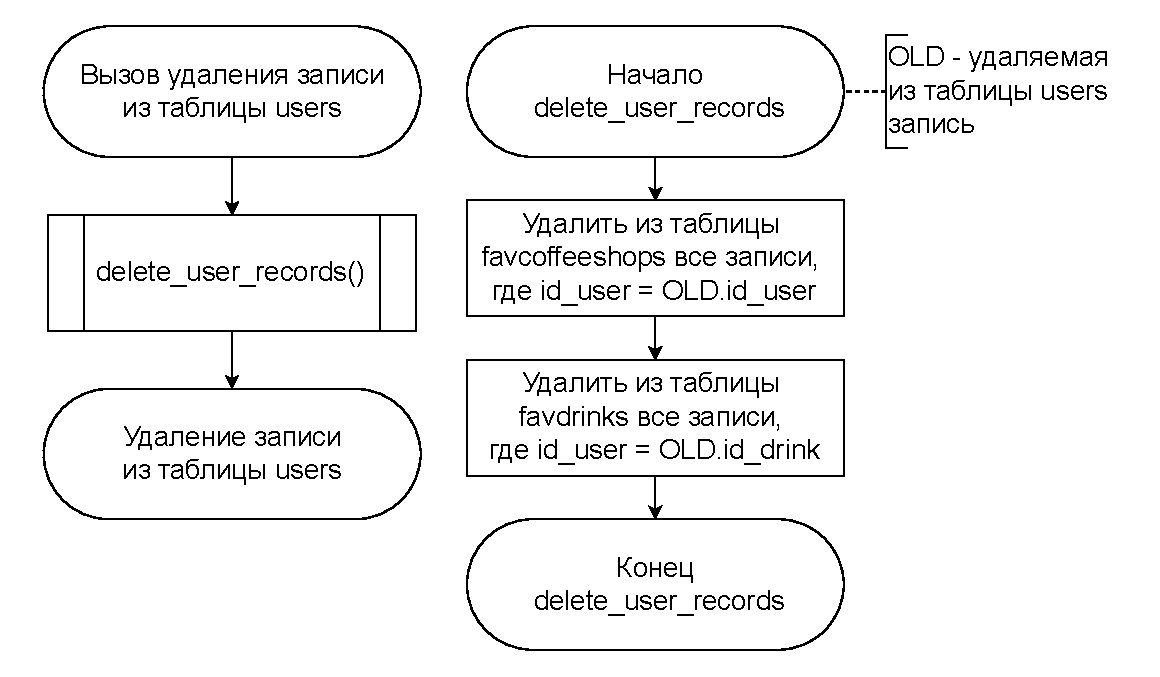
\includegraphics[width=0.7\linewidth]{img/trigger_del_user.pdf}
	\caption{Триггер на удаление всех записей из таблиц  favcoffeeshops и favdrinks, связанных с удаляемым из таблицы users пользователем}
	\label{trigger_del_user}
\end{figure}


Триггер, алгоритм работы которого представлен на рисунке~\ref{trigger_del_coffeeshop}, удаляет из таблицы favcoffeeshops все записи, связанные с удаляемой из таблицы coffeeshops кофейней.

\begin{figure}[H]
	\centering
	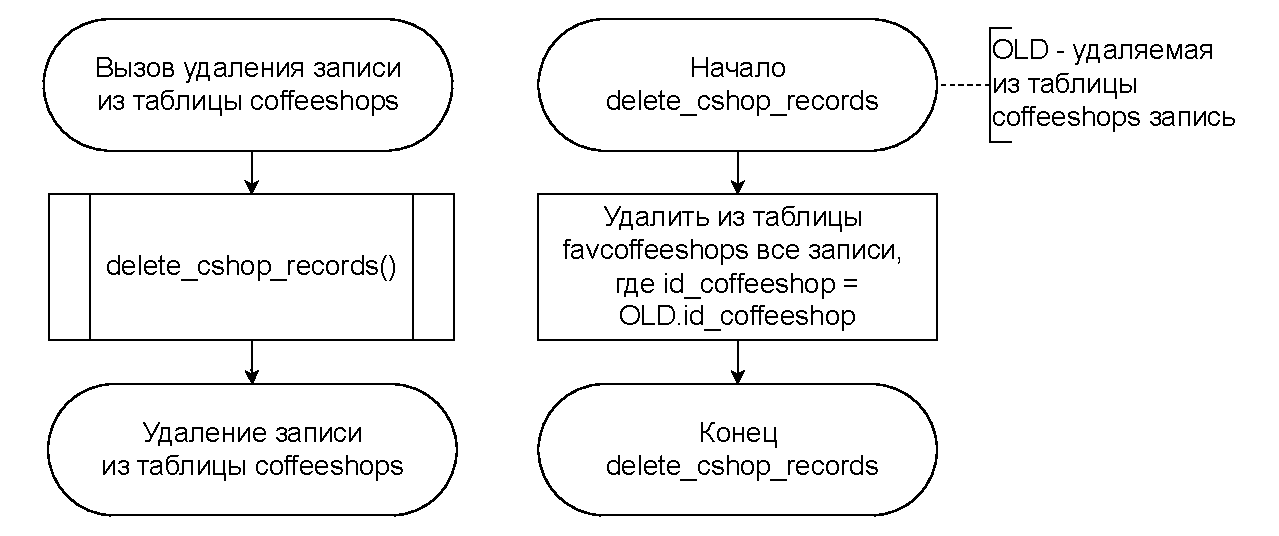
\includegraphics[width=0.8\linewidth]{img/trigger_del_coffeeshop.pdf}
	\caption{Триггер на удаление всех записей из таблицы favcoffeeshops, связанных с удаляемой из таблицы coffeeshops кофейней}
	\label{trigger_del_coffeeshop}
\end{figure}


Помимо описанных выше триггеров необходимо также реализовать триггеры, которые будет увеличивать и уменьшать значение поля amountcoffeeshops записи из таблицы companies при добавлении в таблицу coffeeshops кофейни со значением внешнего ключа, соответствующего первичному ключу упомянутой ранее записи. Алгоритм работы триггера, инкрементирующего значение поля amountcoffeeshops, представлен на рисунке~\ref{increment}, а триггера, декрементирующего это значение, -- на рисунке~\ref{decrement}.

\begin{figure}[H]
	\centering
	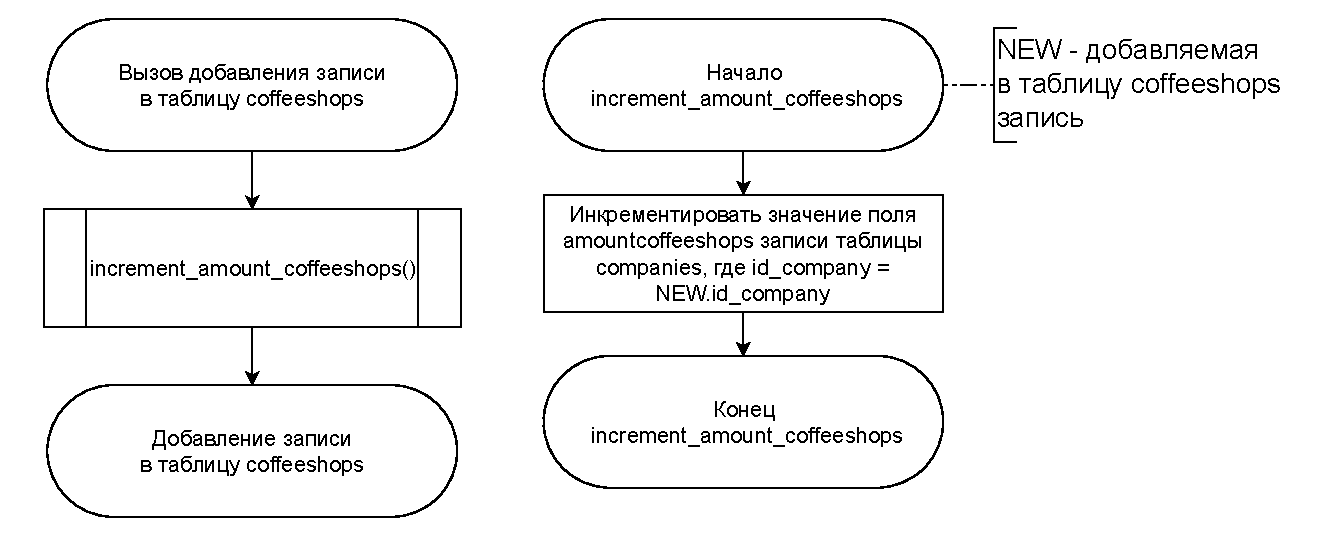
\includegraphics[width=1\linewidth]{img/trigger_incr_amount.pdf}
	\caption{Триггер, инкрементирующий значение поля amountcoffeeshops таблицы companies}
	\label{increment}
\end{figure}


\begin{figure}[H]
	\centering
	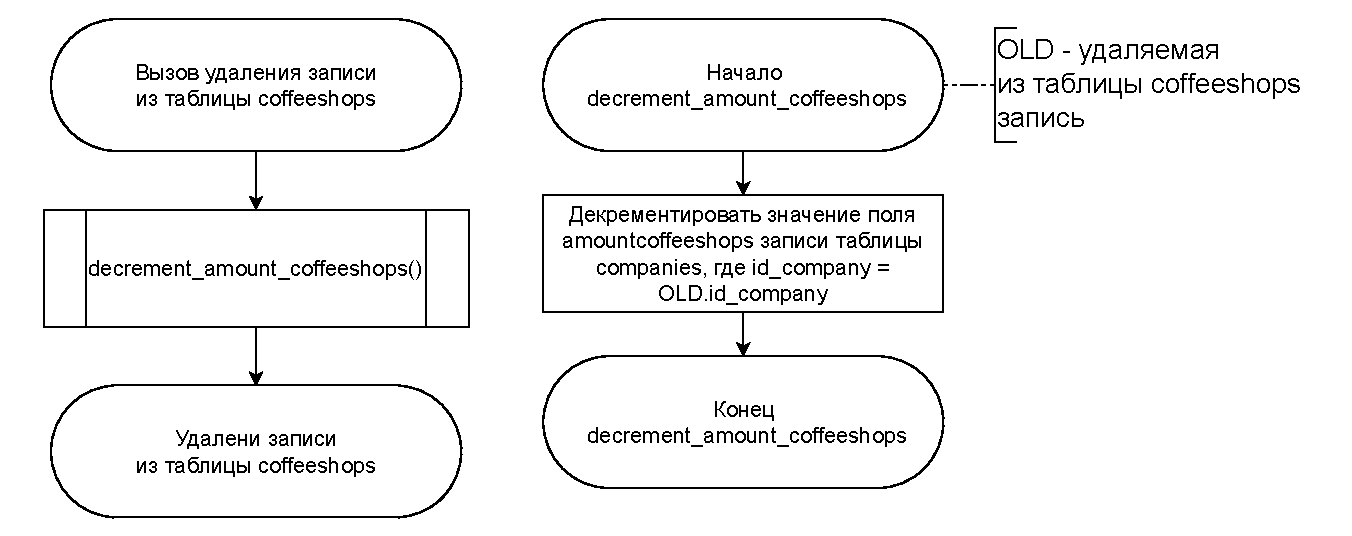
\includegraphics[width=1\linewidth]{img/trigger_decr_amount.pdf}
	\caption{Триггер, декрементирующий значение поля amountcoffeeshops таблицы companies}
	\label{decrement}
\end{figure}

\section{Функции}
Для поиска по идентификатору напитка сетей кофеен, в меню которых представлен данный напиток, определена функция companies\_by\_drink. Алгоритм этой функции представлен на рисунке~\ref{func_find_comp}.


\begin{figure}[H]
	\centering
	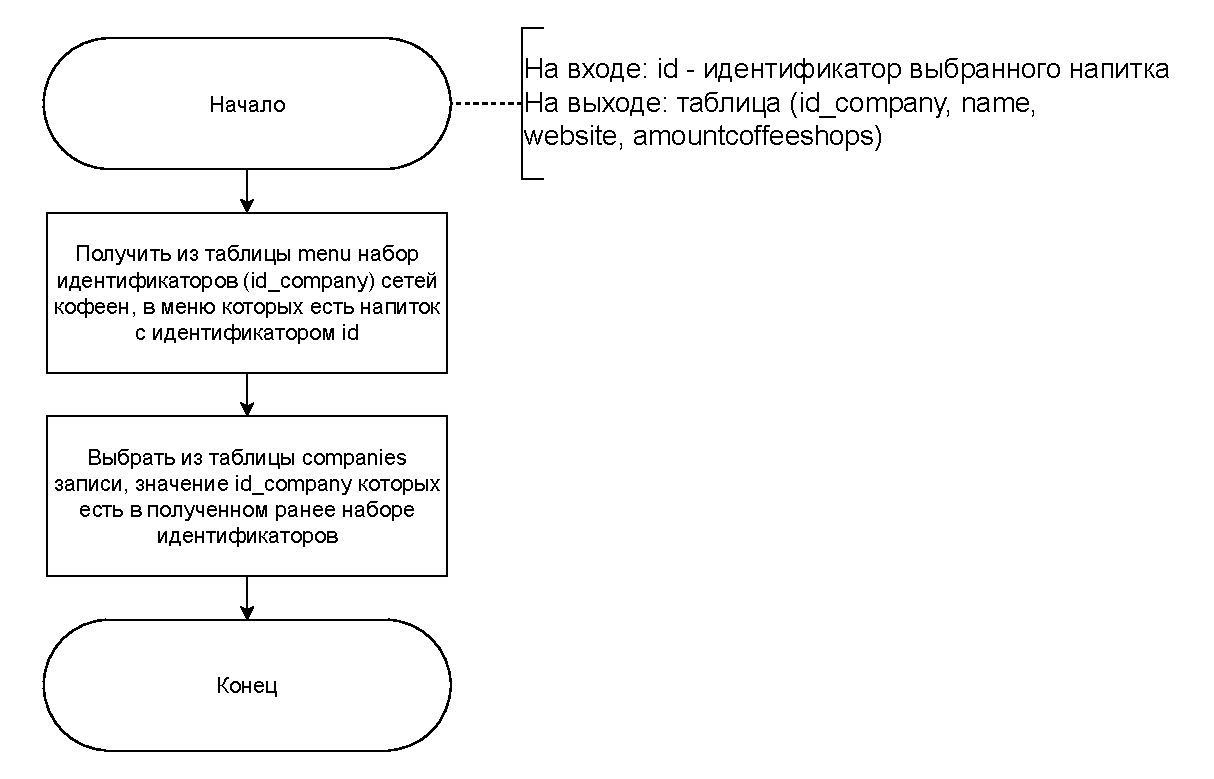
\includegraphics[width=1\linewidth]{img/func_find_companies.pdf}
	\caption{Функция поиска сетей кофеен, в меню которых есть выбранный пользователем напиток}
	\label{func_find_comp}
\end{figure}

Для изменения прав доступа пользователя определена хранимая процедура update\_user\_rights. Алгоритм этой процедуры представлен на рисунке~\ref{proc_moder}.
\begin{figure}[H]
	\centering
	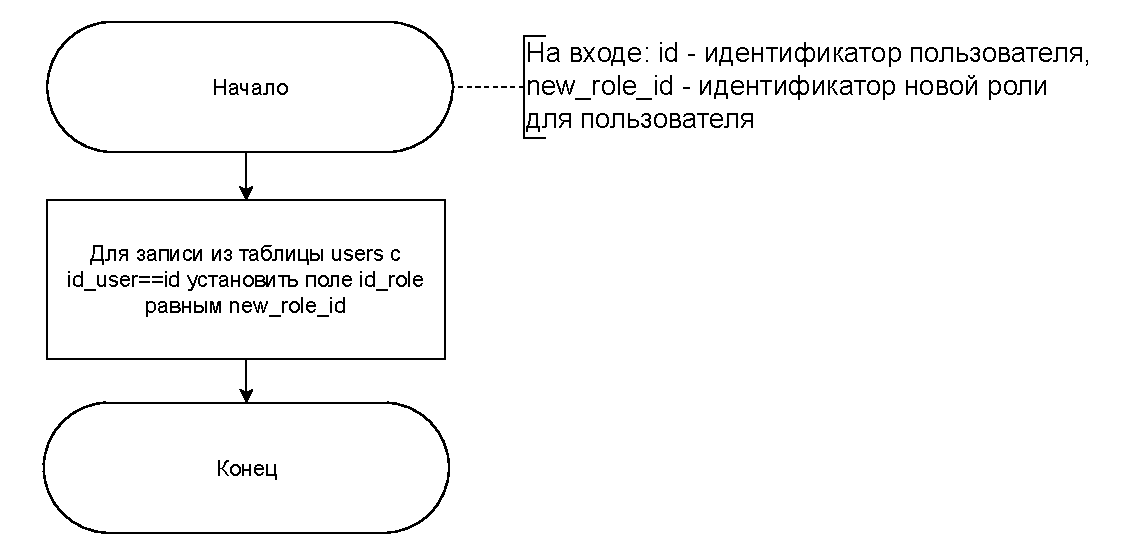
\includegraphics[width=1\linewidth]{img/proc_rights.pdf}
	\caption{Хранимая процедура, выполняющая изменение прав доступа пользователя}
	\label{proc_moder}
\end{figure}


\section{Ролевая модель на уровне базы данных}
В проектируемой базе данных определены следующие роли: гость, обычный пользователь, модератор, администратор.

В соответствии с диаграммой прецедентов, представленной на рисунке~\ref{usecase_all}, \textbf{гостю} выдаются следующие права на таблицы базы данных:
\begin{itemize}
	\item выборка данных из таблиц users, roles;
	\item добавление данных в таблицу users.
\end{itemize}

В соответствии с диаграммой прецедентов, представленной на рисунке~\ref{usecase_all}, \textbf{обычному пользователю} выдаются следующие права на таблицы базы данных:
\begin{itemize}
	\item выборка данных из таблиц users, drinks, companies, coffeeshops, favdrinks, favcoffeeshops, categories, drinkscategory, menu, loyaltyprograms, roles;
	\item добавление данных в таблицы users, favdrinks и favcoffeeshops.
	\item удаление данных из таблиц favdrinks и favcoffeeshops.
	\item обновление данных таблицы users.
\end{itemize}

В соответствии с диаграммой прецедентов, представленной на рисунке~\ref{usecase_all}, \textbf{модератору} выдаются следующие права на таблицы базы данных:
\begin{itemize}
	\item выборка данных из таблиц users, drinks, companies, coffeeshops, favdrinks, favcoffeeshops, categories, drinkscategory, menu, loyaltyprograms, roles;
	\item добавление данных в таблицы users, favdrinks, favcoffeeshops, drinks, menu, coffeeshops, drinkscategory, categories.
		\item удаление данных из таблиц users, favdrinks, favcoffeeshops, drinks, menu, coffeeshops, drinkscategory;
		\item обновление данных таблицы users.
\end{itemize}

В соответствии с диаграммой прецедентов, представленной на рисунке~\ref{usecase_all}, \textbf{администратору} выдаются следующие права на таблицы базы данных:
\begin{itemize}
		\item выборка данных из таблиц users, drinks, companies, coffeeshops, favdrinks, favcoffeeshops, categories, drinkscategory, menu, loyaltyprograms, roles;
	\item добавление данных в таблицы users, favdrinks, favcoffeeshops, drinks, menu, coffeeshops, drinkscategory, categories.
	\item удаление данных из таблиц users, favdrinks, favcoffeeshops, drinks, menu, coffeeshops, drinkscategory;
		\item обновление данных таблицы users.
\end{itemize}




\section*{Вывод}
В данной части были спроектированы таблицы базы данных, описаны ограничения целостности, проектируемые триггеры и функции, а также представлена ролевая модель на уровне базы данных.